% Author: Izaak Neutelings (May 2018)
% Inspiration: https://tex.stackexchange.com/questions/113900/draw-polarized-light
\documentclass[border=3pt,tikz]{standalone}
\usepackage{amsmath} % for \text
\usepackage{tikz}
\usepackage{physics}
\tikzset{>=latex} % for LaTeX arrow head
\usepackage{xcolor}
\usetikzlibrary{3d} % for "canvas is yz plane at x="

\colorlet{vcol}{green!50!black}
\colorlet{Hcol}{green!60!black!80}
\colorlet{Scol}{red!60!orange!80!black!80}
\def\tick#1#2{\draw[thick] (#1) ++ (#2:0.2) --++ (#2-180:0.4)}

\begin{document}


% COST FUNCTIONS
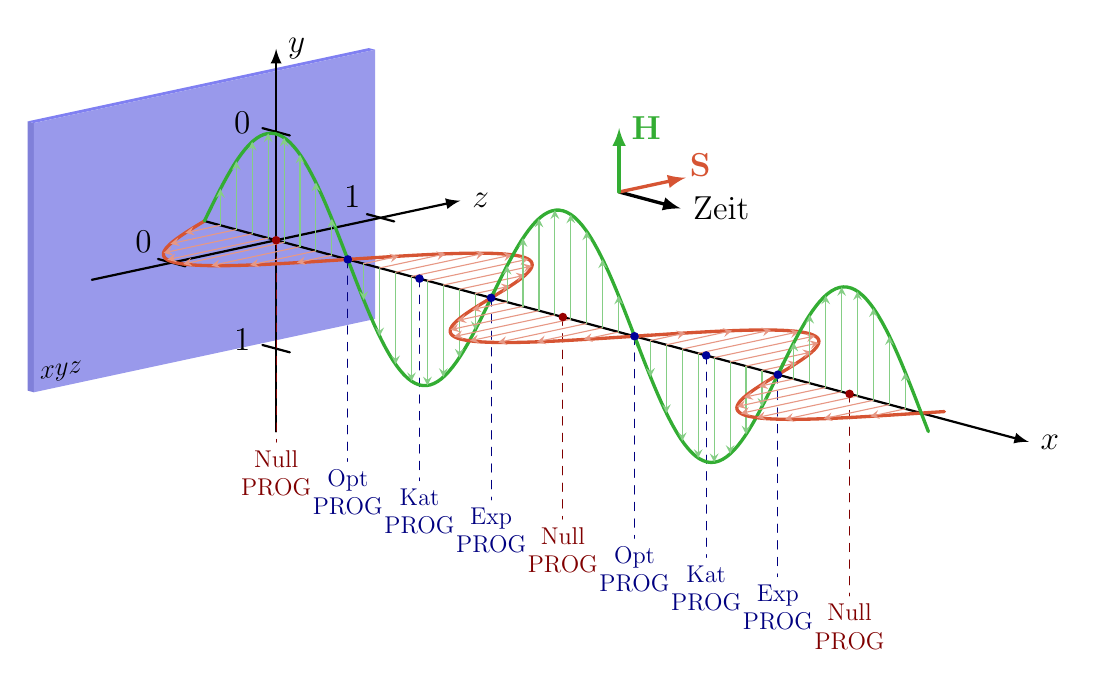
\begin{tikzpicture}[x=(-15:0.9), y=(90:0.9), z=(-155:1.1),
                    line cap=round, line join=round,
                    axis/.style={black, thick,->},
                    vector/.style={>=stealth,->},
                    system/.style={below,align=center,scale=0.73}] %,yslant=tan(-20)
  \large
  \def\A{1.5}                  % amplitude
  \def\nNodes{5}               % use even number
  \def\nVectorsPerNode{8}      % number of vectors per node
  \def\omeg{1.5}               % angular frequency
  \def\xmax{\nNodes*pi/\omeg*1.15}
  \def\ymax{1.8*\A}
  \def\zmax{1.8*\A}
  \def\quart{pi/2/\omeg}       % quarter wavelength for origin shift
  \pgfmathsetmacro\nVectors{(\nVectorsPerNode+1)*\nNodes}
  %\coordinate (O) at (pi/2/\omeg,0,0); % origin
  
  % HELP MACROS
  \def\drawENode{ % draw E node and vectors with some offset
    \draw[Hcol,very thick,variable=\t,domain=\iOffset*pi/\omeg:(\iOffset+1)*pi/\omeg*1.01,samples=40]
      plot (\t,{\A*sin(\omeg*\t*180/pi)},0);
    \foreach \k [evaluate={\t=\k*pi/\omeg/(\nVectorsPerNode+1);
                           \angle=\k*90/(\nVectorsPerNode+1);}]
                in {1,...,\nVectorsPerNode}{
      \draw[vector,Hcol!60]  (\iOffset*pi/\omeg+\t,0,0) --++ (0,{\A*sin(2*\angle+\iOffset*180)},0);
    }
  }
  \def\drawBNode{ % draw B node and vectors with some offset
    \draw[Scol,very thick,variable=\t,domain=\iOffset*pi/\omeg:(\iOffset+1)*pi/\omeg*1.01,samples=40]
      plot (\t,0,{\A*sin(\omeg*\t*180/pi)});
    \foreach \k [evaluate={\t=\k*pi/\omeg/(\nVectorsPerNode+1);
                           \angle=\k*90/(\nVectorsPerNode+1);}]
                in {1,...,\nVectorsPerNode}{
      \draw[vector,Scol!60]  (\iOffset*pi/\omeg+\t,0,0) --++ (0,0,{\A*sin(2*\angle+\iOffset*180)});
    }
  }
  
  % PLATE
  \def\py{1.9} % plate half-width
  \def\pz{2.5} % plate half-height
  \def\t{0.09} % plate thickness
  \fill[blue!70!black!50,canvas is yx plane at z=\pz]
    (-\py,0) rectangle (\py,-\t);
  \fill[blue!90!black!50,canvas is xz plane at y=\py]
    (0,-\pz) rectangle (-\t,\pz);
  \fill[blue!80!black!40,canvas is yz plane at x=0]
    (-\py,-\pz) rectangle (\py,\pz);
  %\draw (\quart,0,\A)--(0,0,\A);
  %\draw (\quart,0,-\A)--(0,0,-\A);
  \node[above right=-1,yslant=tan(10),scale=0.8] at (0,-\py,\pz) {$xyz$};
  
  % MAIN AXES
  \draw[axis] (-0.0*\xmax,0,0) -- (\xmax,0,0) node[right] {$x$};
  \draw[axis] (\quart,-\ymax,0) -- (\quart,\ymax,0) node[right] {$y$};
  \draw[axis] (\quart,0,\zmax) -- (\quart,0,-\zmax) node[right] {$z$};
  \tick{\quart,0,1.02*\A}{0} node[above left=-2] {$0$};
  \tick{\quart,0,-1.02*\A}{0} node[above left=-2] {$1$};
  \tick{\quart,1.02*\A,0}{0} node[above=2,left] {$0$};
  \tick{\quart,-1.02*\A,0}{0} node[above=2,left] {$1$};
  
  % SMALL AXES
  \def\xOffset{{(\nNodes-2)*pi/2}}
  \def\yOffset{\A*0.9}
  \def\zOffset{\A*0.9}
  \draw[axis,very thick,black] (\xOffset,\yOffset,-\zOffset) --++ (\A*0.6,0,0) node[right,align=center] {Zeit}; %\\propagation
  \draw[axis,very thick,Scol]   (\xOffset,\yOffset,-\zOffset) --++ (0,0,-\A*0.65) node[below=1,above right=-3] {$\vb{S}$};
  \draw[axis,very thick,Hcol]  (\xOffset,\yOffset,-\zOffset) --++ (0,\A*0.6,0) node[right] {$\vb{H}$};
  
  % GRAMMATICAL SYSTEMS
  \def\r{1.1}    % dot radius
  \def\d{1.9*\A} % node depth
  \def\nDots{9}  % number of dots
  \foreach \i in {1,...,\nDots}{
    %\fill (\i*\quart,0,0) circle (\r) coordinate (N\i);
    \coordinate (N\i) at (\i*\quart,0,0);
  }
  \draw[dashed,red!50!black] (N1) --++ (0,-\d,0) node[system] {Null\\PROG};
  \draw[dashed,blue!50!black] (N2) --++ (0,-\d,0) node[system] {Opt\\PROG};
  \draw[dashed,blue!50!black] (N3) --++ (0,-\d,0) node[system] {Kat\\PROG};
  \draw[dashed,blue!50!black] (N4) --++ (0,-\d,0) node[system] {Exp\\PROG};
  \draw[dashed,red!50!black] (N5) --++ (0,-\d,0) node[system] {Null\\PROG};
  \draw[dashed,blue!50!black] (N6) --++ (0,-\d,0) node[system] {Opt\\PROG};
  \draw[dashed,blue!50!black] (N7) --++ (0,-\d,0) node[system] {Kat\\PROG};
  \draw[dashed,blue!50!black] (N8) --++ (0,-\d,0) node[system] {Exp\\PROG};
  \draw[dashed,red!50!black] (N9) --++ (0,-\d,0) node[system] {Null\\PROG};
  
  % DRAW (ANTI-)NODES
  \foreach \iNode [evaluate={\iOffset=\iNode-1;}] in {1,...,\nNodes}{
    \ifodd\iNode \drawBNode \drawENode % E overlaps B
    \else        \drawENode \drawBNode % B overlaps E
    \fi
  }
  
  % DOTS (draw on top of nodes)
  \foreach \i [evaluate={\f=100*int(mod(\i,4)==1);}] in {1,...,\nDots}{
    %\fill (N\i) circle (\r);
    \node[fill=red!\f!blue!60!black,circle,inner sep=\r] at (N\i) {};
  }
  
\end{tikzpicture}




\end{document}